\section{Transactions} 

  So far, we've had one query/update on one machine, but this is not the case in reality. In modern systems, you have users interacting with a database all the time and databases may be prone to failure. These two situations requires us to develop a safer way of interacting with the database. 

  \begin{example}[Simultaneous Interaction]
    In an airline, say that we have two parties A and B trying to book the same seat. A looks at the website, which queries the tuple representing the seat. B does the same. A and B then both book it at the same time, sending an update request to the database, causing an overbooking. 

    In a bank, say that we have some events that must be recorded in a database. Say that $A = 0$ and $B = 100$. 
    \begin{enumerate}
      \item T1. B sends \$100 to A. So $A \mapsto A + 100, B \mapsto B - 100$. 
      \item T2. The bank sends all users an interest of 6\%. $A \mapsto 1.06 A, B \mapsto 1.06B$. 
    \end{enumerate}
    This is sensitive to order and perhaps at the end we expect $A = 100$. Consider the following cases. 
    \begin{enumerate} 
      \item $A \mapsto A + 100, B \mapsto B - 100, A \mapsto 1.06A, B \mapsto 1.06B$. This is fine. 
      \item $A \mapsto A + 100, A \mapsto 1.06A, B \mapsto 1.06B, B \mapsto B - 100$. This is not fine since both A and B got interest and the bank lost \$6. 
    \end{enumerate}
  \end{example}

  \begin{example}[Database Crash]
    If $A \mapsto A + 100$ happened first and the bank crashed, then the system would find that $A$ just gained \$100! This is clearly not good, so we must undo what we have done so far. 
  \end{example}

  These two examples hint at some nice properties that we want in our database. 
  \begin{enumerate}
    \item \textit{Serializability}. The first example shows that we do not like parallelism and rather we want things to run \textit{serially} in a way such that T1 and T2 occur separately, like a mutex lock. In practice, there are so many requests that parallelism is a must, so we must find ways to not run serially, but to modify our parallel computing to make it serializable, as if it is running serially.  
    \item \textit{Atomicity}. The second example shows that we want these operations to be \textit{atomic}, i.e. it is fully done or not done at all. That is, we do not want to update the disk (which preserves its state upon powering off) until  T1 is completely finished. A simple solution is to do all the operations in memory (which is wiped upon crashing anyways) and then \textit{commit} (announce that it is done) these changes. \footnote{Committing is not the same as disk writing, actually. It is not necessarily the case that one follows the other, so you can commit before writing and write before committing. There can also be some completed transactions with updated data still in memory and therefore lost in crash.} 
  \end{enumerate} 

  Great, so let's review some actions that our DBMS should support. To read/write some tuple or relation $X$, the disk block containing $X$ must first be brought into memory. $X$ is read/written in memory. If it is written, it is called a \textbf{dirty block}. Finally, this dirty block must be flushed to disk. 

  \begin{definition}[Actions]
    Some examples of actions that can occur in a schedule is: 
    \begin{enumerate}
      \item \texttt{READ}: read in a memory block from disk
      \item \texttt{WRITE}: write/flush out a dirty memory block 
      \item \texttt{COMMIT}
      \item \texttt{ABORT} 
    \end{enumerate}
    Note that committing is not the same as writing! 
  \end{definition}

  \begin{definition}[Transaction]
    The solution to both serializability and atomicity is to use \textbf{transactions}, which is a collection of one or more operations, called \textbf{actions}, on the database that must be executed atomically as a whole. At the end of every transaction, the DBMS always puts either a commit (indicating successful completion) or abort signal. 
  \end{definition} 

  \begin{definition}[Schedule]
    Now that we've cleared up on transactions, a schedule is simply a sequence of actions gotten from interweaving the transactions on the DBMS. It must obviously be consistent, and two actions from the same transaction T must appear in the schedule in the same order that they appear in T. Some terminology to compare schedules: 
    \begin{enumerate}
      \item \textbf{Serial Schedule}. No interweaving of transactions. 
      \item \textbf{Equivalent Schedule}. Two schedules that have the same effect on the database state after completion. 
      \item \textbf{Serializable Schedule}. A schedule that is equivalent to a serial schedule. 
    \end{enumerate}
    In a schedule, the transactions are usually written in $T, S, \ldots$ and they act on \textbf{elements} (data, tuples or relations, on disk or memory). 
  \end{definition}

  \begin{example}[Bank Schedule]
    For the bank example above, we can construct a serial schedule $S_1$. 
    \begin{lstlisting}
      T1: R(A) W(A) R(B) W(B) C(T1)
      T2:                           R(A) W(A) R(B) W(B) C(T2)

      T:  R1(A) W1(A) R1(B) W1(B) C(T1) R2(A) W2(A) R2(B) W2(B) C(T2)
    \end{lstlisting}
    and a serializable schedule $S_2$. 
    \begin{lstlisting}
      T1: R(A) W(A)           R(B) W(B) C(T1) 
      T2:           R(A) W(A)                 R(B) W(B) C(T2)
      T:  R1(A) W1(A) R2(B) W2(B) R1(B) W1(B) C(T1) R2(B) W2(B) C(T2)
    \end{lstlisting}
    We can verify that $S_1 \equiv S_2$ since in the second transaction, we always read in A after it is written by the first transaction. However, the following is not a serializable schedule since T2 reads the unmodified A block from disk before flushed by T1.  
    \begin{lstlisting}
      T1: R(A)                           W(A) R(B) W(B) C(T1)
      T2:      R(A) W(A) R(B) W(B) C(T2)
    \end{lstlisting}
  \end{example} 

  These properties are a subset of the general ones described here. In the next sections, we will go over implementing features that ensure each of these properties. 

  \begin{definition}[ACID]
    These properties are a subset of the \textbf{ACID} properties.
    \begin{enumerate}
      \item \textit{Atomicity}. A user can think of a transaction as always executing all actions in one stop or not executing any at all. In an abort, this can be undone by storing recovery logs and going through the history to undo. 
      \item \textit{Consistency}. Each transaction, when run by itself with no concurrent execution of other actions, must preserve the consistency of the database.\footnote{e.g. if you transfer money from one account to another, the total amount in circulation still remains the same. The constraints must also be maintained. } 
      \item \textit{Isolation}. A user should be able to understand a transaction without considering the effect of any other concurrently running transaction. This allows us to have \textit{concurrency control}, which handles multiple transactions by interweaving them in a serializable way (like the bank example we saw above), and sometimes they may ensure isolation with locks.  

      \item \textit{Durability}. Once the DBMS informs the user that a transaction is completed, its effect should persist.\footnote{Even if the system crashes before writing to disk, we can recover it by using the history logs and redoing them.}
    \end{enumerate}

    It turns out that making one stricter usually leads to a decrease in performance in the other, so we should maintain some balance. C/I are usually improved in conjunction with concurrency controls, and A/D are improved using recovery. 
  \end{definition}

\subsection{Consistency: Serizability and Precedence Graph}

  Okay, so we've seen in the bank schedule example that serial schedules are trivial to construct and ideally we want to construct serializable schedules. How do we detect them? Well it turns out checking for serializability is NP-complete, so we must resort to something called \textit{conflict-serializability}, which is a stronger condition but can be solved in polynomial time. Conflict-serializability assures the absence of \textit{conflicts}, which are certain properties of schedules that result in a corrupt schedule.   

  \begin{definition}[Conflict]
    When we interweave actions, \textbf{conflicts} cause schedules to be not equivalent to the serial schedule. There are 3 types of conflicts. 
    \begin{enumerate}
      \item Write-Read (WR): $T_1$ writes $A$ and then $T_2$ reads $A$ before $T_1$ commits. This causes reading uncommitted (dirty) data. 
      \item Read-Write (RW): $T_1$ reads $A$ and then $T_2$ writes $A$ before $T_1$ commits. This causes unrepeatable reads. 
      \item Write-Write (WW): $T_1$ writes $A$ and then $T_2$ writes $A$ before $T_1$ commits. This overwrites uncommitted data or lost updates. 
      \item 
    \end{enumerate}
    Note that RR (read read) has no conflicts since there are no writes. 
  \end{definition}

  We can make a \textit{precedence graph}. 

  \begin{definition}[Precedence Graph]
    A \textbf{precedence graph} contains 
    \begin{enumerate}
      \item a node for each transaction 
      \item a directed edge from $T_i$ to $T_j$ if an operation of $T_i$ precedes and conflicts with an operation of $T_j$ in the schedule. 
    \end{enumerate}
  \end{definition} 

  \begin{example}[Precedence Graph]
    Consider the following schedule between 2 transactions. 
    \begin{lstlisting}
      R1(A) R2(A) W1(A) C1 C2
    \end{lstlisting}
    Then, our precedence graph $G(V, E)$ is defined $V = \{T_1, T_2\}$ and $E = \{(T_2, T1)\}$ since there is a RW conflict. Now consider the following. 
    \begin{lstlisting}
      R1(A) R2(A) W1(A) W2(A) C1 C2
    \end{lstlisting}
    Its precedence graph has both edges $(T_1, T_2)$ due to \texttt{R1(A)...W2(A)} and $(T_2, T_1)$ due to \texttt{R2(A) W1(A)}. 
  \end{example}

  \begin{theorem}[Conflict-Serializability]
    A schedule is \textbf{conflict-serializable} (which implies serizability) if its precedence graph is acyclic. 
  \end{theorem} 

  \begin{example}[Not Serializable]
    The following schedule is not conflict serializable since $T_1 \mapsto T_2$ from the transactions on $A$ and $T_2 \mapsto T_1$ from the transactions on $B$. 
    \begin{lstlisting}
      T1: R(A) W(A)                     R(B) W(B)
      T2:           R(A) W(A) R(B) W(B) 
    \end{lstlisting}
  \end{example}

  We established a method to check if a certain schedule $S_1$ is conflict-serializable. Given two serial schedules $S_1, S_2$, we can check if they are equivalent serial schedules as well. 

  \begin{theorem}[Equivalent Serial Schedules]
    Given 2 serial schedules $S_1, S_2$, let $G_1, G_2$ be their precedence graphs. If $G_1$ and $G_2$ have a common existing topological ordering, then $S_1 \equiv S_2$. 
  \end{theorem} 

  \begin{theorem}[Swapping Non-Conflicting Actions Doesn't Change Precedence Graph]
    You can also swap adjacent non-conflicting actions to reach an equivalent serial schedule. 

    \begin{figure}[H]
      \centering 
      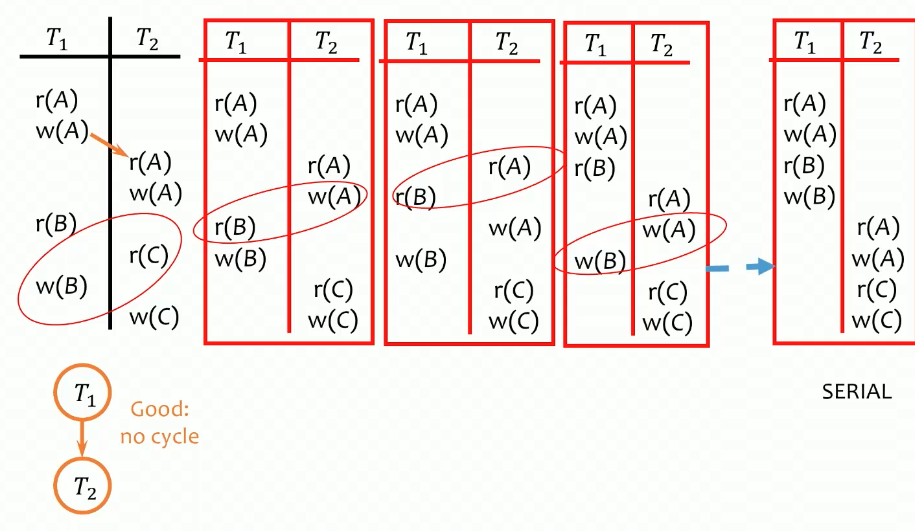
\includegraphics[scale=0.4]{img/swap_serial.png}
      \caption{You can first swap W(B) and R(C) since they act on different elements. You keep swapping to push the actions of T1 up as far as possible, and if you can get a serial schedule, you are good. Swapping non-conflicting actions does not affect the precedence graph of the schedule(?)} 
      \label{fig:swap_serial}
    \end{figure}
  \end{theorem} 

\subsection{Isolation and Concurrency Control} 

    We've seen that ideally, we would like to have a schedule that is conflict-serializable. The avoiding of conflicts is just one problem that we must avoid when implementing isolation protocols, and in here we will focus on implementing a protocol that enforces three properties: 
    \begin{enumerate}
      \item conflict-serializability 
      \item avoiding cascading rollbacks 
      \item recoverability
    \end{enumerate}
    While looking at precedence graphs allow us to compare already existing schedules, it does not give us instructions to \textit{create} one. We can do this using locks. 

  \subsubsection{Locks}

    Let's introduce locks in the basic sense. 

    \begin{definition}[Locks]
      The rules for \textbf{locks} are as follows: 
      \begin{enumerate}
        \item If a transaction wants to read an object, it must request a \textbf{shared lock} (S mode) on that object. 
        \item If a transaction wants to read/modify an object, it must first request an \textbf{exclusive lock} (X mode) on that object. 
        \item You can allow one exclusive lock, or multiple shared locks. 
      \end{enumerate}
    \end{definition}

    \begin{example}[Basic Locking]
      An implementation of basic locking is shown below. 
      \begin{lstlisting}
        T1: X(A) R(A) W(A) U(A)                                         X(B) R(B) W(B) U(B) 
        T2:                     X(A) R(A) W(A) U(A) X(B) R(B) W(B) U(B) 
      \end{lstlisting}
    \end{example}

    However, notice that basic locking does not really enforce conflict-serializability. Naive locks still allow for this non-serializable schedule to occur. Therefore, we can do two-phase locking. 

    \begin{definition}[Two-Phase Locking (2PL)]
      The basic rule is that \textit{for each individual transaction}, all lock requests precede all unlock requests. Therefore, every transaction is divided into a phase of obtaining locks and releasing locks.   
    \end{definition}

    \begin{example}[2PL]
      Look at this previous schedule. 
      \begin{lstlisting}
        T1: R(A) W(A)                     R(B) W(B)
        T2:           R(A) W(A) R(B) W(B) 
      \end{lstlisting}
      \begin{enumerate}
        \item T1 will first requests a $X$ lock on $A$. 
        \item Then T2 wants to write to $A$ so it must have the lock. In order to do this T1 must unlock $A$, but as soon as it unlocks $A$, it cannot request for any more locks. What can it do? It has no choice but to request for a lock on $B$ \textit{now}, and then unlock $A$ to give to T2. 
        \item T2 unlocks $A$, reads/writes it, and then wants to unlock $A$, but again it must request $B$ before unlocking $A$. However, T1 already holds the lock on $B$ and cannot unlock it since it must write $B$ later. 
      \end{enumerate}
      \begin{lstlisting} 
        T1: X(A) R(A) W(A) X(B) U(A) 
        T2:                          X(A) R(A) W(A) ... not allowed
      \end{lstlisting}
      This block really comes from the fact that this schedule is not serializable. Consider a serializable schedule instead. 
      \begin{lstlisting} 
        T1: R(A) W(A)           R(B) W(B)
        T2:           R(A) W(A)           R(B) W(B) 
      \end{lstlisting} 
      Then we can construct the 2P locks as such. 
      \begin{lstlisting}
        T1: X(A) R(A) W(A) X(B) U(A)                R(B) W(B) U(B) 
        T2:                          X(A) R(A) W(A)                X(B) U(A) R(B) W(B) U(B) 
      \end{lstlisting}
      Fundamentally, what we are trying to do by having all locks come first is to push all actions on $A$ (and their associated locks) as far up as possible so we can finish them first. By pushing them up, we can isolate $R$ and not have two-way conflicts between T1 and T2. 
    \end{example}

    2PL is great, but we still have to look at the remaining two desired properties. Let's show why it doesn't satisfy them. 

    \begin{example}[Cascading Rollback and Irrecoverability in 2PL]
      Consider the following problems with 2PL.  
      \begin{enumerate}
        \item Say that T1 is reading $A$ and adds 5 to it to write. Then T2 will read $A=10$ and double it for write. If T1 decides to abort before writing, it should look like T1 had never happened, so T2 should have been reading $A=5$. This is problematic, and the only way to deal with this is to abort T2 as well. If there are other transactions, this is called a \textbf{cascading rollback}. 
          \begin{lstlisting}
            T1: R(A=5) W(A=10)         Abort 
            T2:                R(A=10)       W(A=20) Must abort T2
          \end{lstlisting}

        \item A schedule may not be recoverable sometimes. We can see that T1 aborts, but by the time it aborts, it's too late: T2 had already committed changes using uncommitted data from T1, which must now be undone. 
          \begin{lstlisting}
            T1: R(A=5) W(A=10)                        Abort
            T2:                R(A=10) W(A=20) Commit
          \end{lstlisting}
      \end{enumerate}
    \end{example}

    Therefore, we would like to 
    \begin{enumerate}
      \item \textit{Avoid cascading rollbacks}. All transactions should only read data by committed transactions. 
      \item \textit{Recoverable}. A transaction commits only after all transactions it had read from commits. 
    \end{enumerate} 
    By enforcing even stricter conditions, we can get this as well. 

    \begin{definition}[Strict 2PL]
      \textbf{Strict 2PL} only releases locks at commit/abort time. A writer will block all other readers until the writer commits or aborts.
    \end{definition}

    \begin{example}[2PL vs Strict 2PL]
      Consider the following schedule. 
      \begin{lstlisting}
        T1: X(A) W(A) U(A)                C
        T2:                X(A) W(A) U(A)   C
      \end{lstlisting}
      \begin{enumerate}
        \item 2PL allows this schedule since for each transaction, all unlocks come after all locks. 
        \item Strict 2PL does not allow this schedule since it asserts that you must commit before unlocking (and having other transactions use the lock). 
      \end{enumerate} 
      With strict 2PL, you must use this schedule, which requires the commits to be before the transaction. 
      \begin{lstlisting}
        T1: X(A) W(A) C U(A) 
        T2:                  X(A) W(A) C U(A)
      \end{lstlisting}
    \end{example}

    It seems that we are regressing more and more back to the serial schedule, and yes this is true. By enforcing stricter conditions, we are forced to isolate more and more until it is serial. However, this is used in many commercial DBMS because reliability is often more important than efficiency.\footnote{Oracle is a notable exception.} 

  \subsubsection{Snapshots} 
    
    Oracle uses snapshot isolation. Covered in 516. It uses a private snapshot or a local copy. If there are no conflicts, it makes global changes and aborts otherwise. It is more efficient than locks, but may lead to aborts.  

  \subsubsection{Timestamp-Based Concurrency Control} 
    
    

  \subsubsection{Conflicts and Isolation Levels}

    We can actually enforce isolation levels in SQL directly. In SQL a transaction is automatically started when a user executes a SQL statement, and subsequent statements in the same session are executed as part of this transaction. Statements see changes made by earlier ones in the same transaction and statements in other concurrently running transactions do not. \texttt{COMMIT} and \texttt{ROLLBACK} commands are self explanatory.  
     
    SQL also supports isolation levels, which increases performance by eliminating overhead and allowing higher levels of concurrency, albeit at the cost of getting inconsistent answers if you don't know what you're doing. We start off with the most restrictive and go down. 
    \begin{enumerate}
      \item \texttt{SERIALIZABLE} is the strongest isolation level, with complete isolation. 

      \item \texttt{REPEATABLE READ} allows repeated reads, and you are safe with updates, but you aren't safe with new insertions, which are called \textit{phantoms}. 

      \begin{figure}[H]
        \centering 
        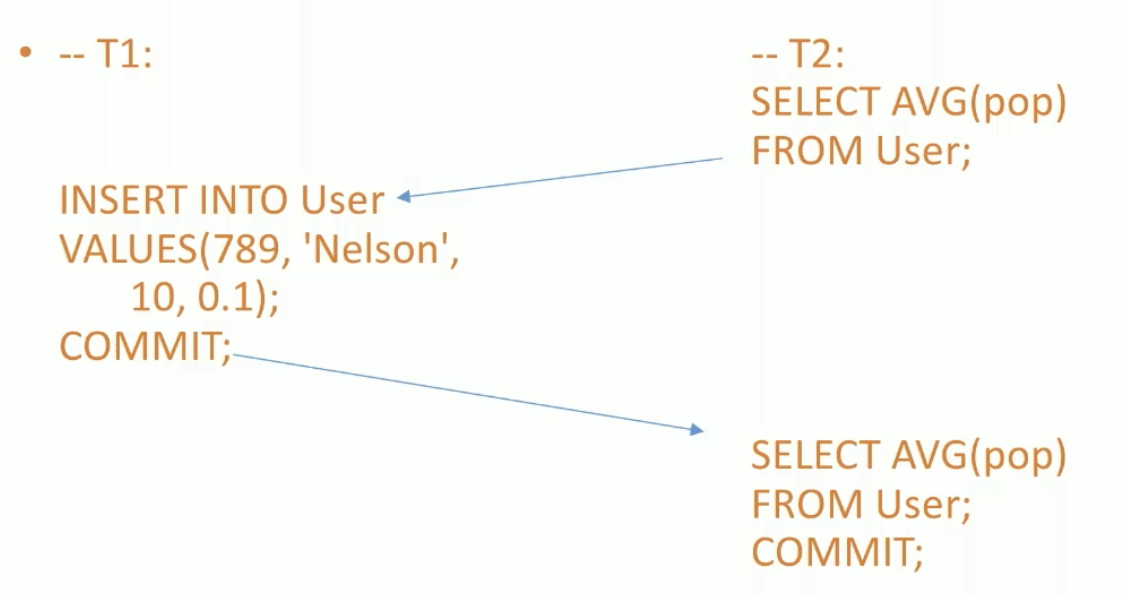
\includegraphics[scale=0.4]{img/rep_read.png}
        \caption{You still have a different average due to the insertion of a new element. } 
        \label{fig:rep_read}
      \end{figure}

      \item \texttt{READ COMMITTED} does not allow dirty reads, but non-repeatable reads are allowed (RW conflicts), which means that reading the same data twice can produce different results and is allowed. 

      \begin{figure}[H]
        \centering 
        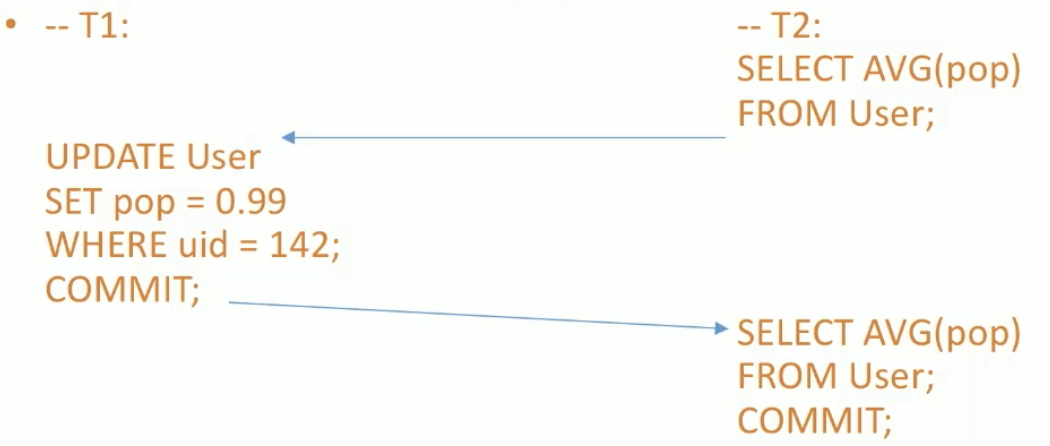
\includegraphics[scale=0.4]{img/read_c.png}
        \caption{In T2, we first compute an average of say 0.6. Then in T1 we update the popularity and commit. Then in T2, we take the average again, getting 0.8, and finally commit. T2 ends up reading two different states of the database.} 
        \label{fig:read_committed}
      \end{figure}

      \item \texttt{READ UNCOMMITTED} allows you to read uncommitted/dirty data (WR conflict). 

      \begin{figure}[H]
        \centering 
        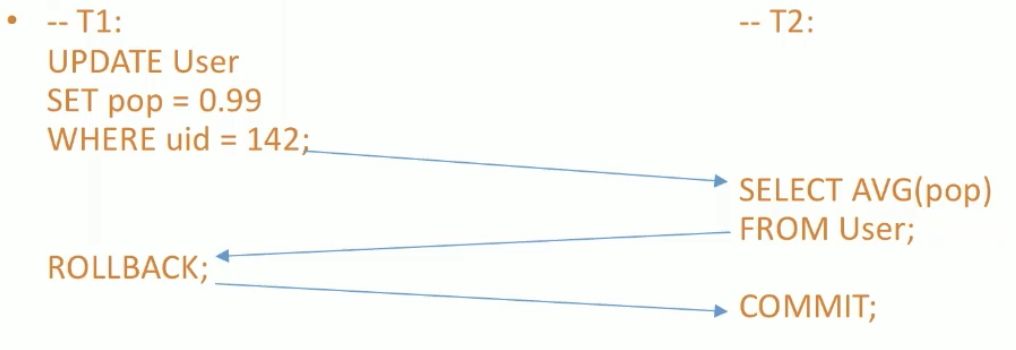
\includegraphics[scale=0.4]{img/read_unc.png}
        \caption{In T1, you are setting the popularity to 0.99. In T2, you read this uncommitted data to compute the average. However, T1 aborts this write, and in T2 you are left with the wrong average. } 
        \label{fig:read_uncommitted}
      \end{figure}
    \end{enumerate}

    Here is a summary of the isolation levels.\footnote{Postgres defaults to read committed.}

    \begin{figure}[H]
      \centering
      \begin{tabular}{|p{5cm}|p{2cm}|p{4cm}|p{2cm}|}
        \hline
        \textbf{Isolation level/anomaly} & \textcolor{orange}{\textbf{Dirty reads}} & \textcolor{orange}{\textbf{Non-repeatable reads}} & \textcolor{orange}{\textbf{Phantoms}} \\
        \hline
        \textcolor{orange}{\textbf{READ UNCOMMITTED}} & Possible & Possible & Possible \\
        \hline
        \textcolor{orange}{\textbf{READ COMMITTED}} & \textcolor{green}{Impossible} & Possible & Possible \\
        \hline
        \textcolor{orange}{\textbf{REPEATABLE READ}} & \textcolor{green}{Impossible} & \textcolor{green}{Impossible} & Possible \\
        \hline
        \textcolor{orange}{\textbf{SERIALIZABLE}} & \textcolor{green}{Impossible} & \textcolor{green}{Impossible} & \textcolor{green}{Impossible} \\
        \hline
      \end{tabular}
      \caption{SQL Transaction Isolation Levels and Possible Anomalies}
      \label{fig:isolation-levels}
    \end{figure}


\subsection{Atomicity and Durability} 

    Note that whenever we read from or write to disk, we are incurring an IO cost and therefore a delay. Since committing and writing to disk are not the same thing, there are two risks: 
    \begin{enumerate}
      \item A system may crash in the middle of transaction $T$ before committing, keeping only partial effects of $T$. This violates atomicity, and we should know how to \textit{undo} $T$. 
      \item A system may crash right after a transaction $T$ commits, and not all effects of $T$ were written to disk. This violates durability, and we should know how to \textit{complete} $T$. 
    \end{enumerate} 

    \begin{example}[No Steal and Force]
      A naive approach to these two risks are as such.  
      \begin{enumerate}
        \item \textit{No steal}. Writes of a transaction can only be flushed to disk at commit time. With steal, if the system crashes before $T$ commits but after some writes of $T$ have been flushed to disk, there is no way to undo these writes. 
        \item \textit{Force}. When a transaction commits, all writes of this transaction must be reflected on disk. Without force, if a system crashes right after $T$ commits, the effects of $T$ will be lost. 
      \end{enumerate}
    \end{example}

  \subsection{Logging} 

    Just as we enforced isolation and concurrency control with locking, we can kill two birds with one stone here with \textit{logging}. 

    \begin{definition}[Log]
      A \textbf{log} is a sequence of \textbf{records} that records all changes made to the database.\footnote{This is stored in a special data structure called \textit{aries}, developed at IBM.} There are 3 types of logs.
      \begin{enumerate}
        \item \texttt{Start}: When a transaction starts, we log 
          \begin{equation}
            \langle T_i, \texttt{start} \rangle
          \end{equation}
        \item \texttt{Write}: When transaction $T$ takes element $A$ and changes value $5$ to $10$, we log 
          \begin{equation}
            (T, A, 5, 10)
          \end{equation}
        \item \texttt{Commit}, \texttt{Abort}: When a transaction $T$ is committed or aborted, we log 
          \begin{equation}
            \langle T_i , \texttt{commit} \rangle \text{ or } \langle T_i , \texttt{abort} \rangle
          \end{equation}
      \end{enumerate}
      Logs are stored in disk (stable storage) and used in recovery. 
      It satisfies \textbf{write-ahead logging (WAL)}, which states that before $A$ is modified in disk, the log record pertaining to $A$ must be flushed. 
    \end{definition}

    At first glance, logging may sound like a bad idea. Since every time we do a transaction, we don't do 1 IO but 2, so this may hurt our performance. However, log writing is really sequential since we're appending to the end of a log only, so we can use dedicated disks with fast append operations to minimize this performance impact. 

    \begin{theorem}[No Force and Seal of Logging]
      Counterintuitively, logging applies no force and steal (as opposed to no steal and force in our naive approach). 
      \begin{enumerate}
        \item \textit{Steal}. Modified memory blocks can be flushed to disk anytime. This is fine since undo information is logged due to WAL. 
        \item \textit{No Force}. A transaction can commit even if its modified memory blocks have not been written to disk. This is fine since redo information is logged due to WAL. 
      \end{enumerate}
    \end{theorem} 

    \begin{example}[Bank Transfer]
      Say that we have two elements/tuples $A = 800, B = 400$ on disk. The schedule is just one transaction that will look something like this. Let $D, L, M$ refer to our main disk, log disk, and memory. 
      \begin{enumerate}
        \item We log that $T$ has started. 

          \noindent\begin{minipage}{.46\textwidth}
            \begin{lstlisting}[]{Code}
              Disk    Memory
              A=800   
              B=400
            \end{lstlisting}
            \end{minipage}
            \hfill
            \begin{minipage}{.45\textwidth}
            \begin{lstlisting}[]{Output}
              Log 
              [T, start]
              .
            \end{lstlisting}
          \end{minipage}

        \item $T$ loads $A=800$ from disk to memory. 

          \noindent\begin{minipage}{.46\textwidth}
            \begin{lstlisting}[]{Code}
              Disk    Memory
              A=800   A=800
              B=400
            \end{lstlisting}
            \end{minipage}
            \hfill
            \begin{minipage}{.45\textwidth}
            \begin{lstlisting}[]{Output}
              Log 
              [T, start]
              .
            \end{lstlisting}
          \end{minipage}

        \item $T$ writes $A=700$ in memory and logs the write at the same time. This is fine since WAL forces logging before \textit{flushing} to disk, not writes on memory. 

          \noindent\begin{minipage}{.46\textwidth}
            \begin{lstlisting}[]{Code}
              Disk    Memory
              A=800   A=700
              B=400
            \end{lstlisting}
            \end{minipage}
            \hfill
            \begin{minipage}{.45\textwidth}
            \begin{lstlisting}[]{Output}
              Log 
              [T, start]
              [T, A, 800, 700]
            \end{lstlisting}
          \end{minipage}

        \item We load $B=400$ into memory. 

          \noindent\begin{minipage}{.46\textwidth}
            \begin{lstlisting}[]{Code}
              Disk    Memory
              A=800   A=700
              B=400   B=400
            \end{lstlisting}
            \end{minipage}
            \hfill
            \begin{minipage}{.45\textwidth}
            \begin{lstlisting}[]{Output}
              Log 
              [T, start]
              [T, A, 800, 700]
            \end{lstlisting}
          \end{minipage}

        \item $T$ writes $B=500$ in memory and logs the write. 

          \noindent\begin{minipage}{.46\textwidth}
            \begin{lstlisting}[]{Code}
              Disk    Memory
              A=800   A=700
              B=400   B=500
              .
            \end{lstlisting}
            \end{minipage}
            \hfill
            \begin{minipage}{.45\textwidth}
            \begin{lstlisting}[]{Output}
              Log 
              [T, start]
              [T, A, 800, 700]
              [T, b, 400, 500]
            \end{lstlisting}
          \end{minipage}

        \item We flush the value of $A$ to disk. Note that by steal, we can flush before committing $T$.  

          \noindent\begin{minipage}{.46\textwidth}
            \begin{lstlisting}[]{Code}
              Disk    Memory
              A=700   A=700
              B=400   B=500
              .
            \end{lstlisting}
            \end{minipage}
            \hfill
            \begin{minipage}{.45\textwidth}
            \begin{lstlisting}[]{Output}
              Log 
              [T, start]
              [T, A, 800, 700]
              [T, b, 400, 500]
            \end{lstlisting}
          \end{minipage} 

        \item We commit $T$, which goes to the log. This marks the end of the transaction. 

          \noindent\begin{minipage}{.46\textwidth}
            \begin{lstlisting}[]{Code}
              Disk    Memory
              A=700   A=700
              B=400   B=500
              .
            \end{lstlisting}
            \end{minipage}
            \hfill
            \begin{minipage}{.45\textwidth}
            \begin{lstlisting}[]{Output}
              Log 
              [T, start]
              [T, A, 800, 700]
              [T, b, 400, 500] 
              [T, commit]
            \end{lstlisting}
          \end{minipage} 

        \item We flush the value of $B$ to disk. Note that by no force, we can flush after committing $T$. Note that this does not log. 

          \noindent\begin{minipage}{.46\textwidth}
            \begin{lstlisting}[]{Code}
              Disk    Memory
              A=700   A=700
              B=500   B=500
              .
            \end{lstlisting}
            \end{minipage}
            \hfill
            \begin{minipage}{.45\textwidth}
            \begin{lstlisting}[]{Output}
              Log 
              [T, start]
              [T, A, 800, 700]
              [T, b, 400, 500] 
              [T, commit]
            \end{lstlisting}
          \end{minipage} 

      \end{enumerate}
    \end{example}

    With this flexibility to flush anytime, we as the programmers really just care about the correctness about the schedule and don't care about the order.  

  \subsubsection{Checkpointing} 
    
    We've seen the advantages of log files, but they can get quite long very fast. If a system crashes and we must recover our operations, it may not be ideal to start the recovery from the beginning of a schedule. Rather, we want to use \textit{checkpointing}. Let's go through a naive approach. 

    \begin{definition}[Naive Checkpointing]
       To checkpoint, 
       \begin{enumerate}
         \item we stop accepting new transactions 
         \item finish all active transactions 
         \item take a database dump
       \end{enumerate}
       To recover, we can start from the last checkpoint. 
    \end{definition} 

    We can already see a few problems with this approach, especially the performance impact on not accepting new transactions. Therefore, we use a more sophisticated approach. 

    \begin{definition}[Fuzzy Checkpointing]
      To place a fuzzy checkpoint, we do the following. 
      \begin{enumerate}
        \item We determine $S$, the set (ids of) currently active transactions. 
        \item We log $\langle \texttt{START CKPT S} \rangle$ 
        \item We flush all dirty blocks up to the checkpoint to disk (however, actions within the checkpoint may or may not get flushed within the checkpoint). 
        \item Transactions normally proceed and new transactions can start during checkpointing. 
        \item We log $\langle \texttt{END CKPT START-CKPT\_location} \rangle$, where the start checkpoint location allows you to easily access the location of the start (otherwise we can read the log backwards to find it). 
      \end{enumerate}
      Now once a bad event like a crash happens, there are three recovery steps. 
      \begin{enumerate}
        \item \textit{Analysis}. Go backward from crash point. 
        \item \textit{Repeating History}. Forward takes care of REDO for committed transactions. 
        \item \textit{UNDO}. Backward takes care of UNDO of uncommitted transactions and removes their effects. 
      \end{enumerate}
    \end{definition} 

    \begin{example}[Crash After T2]
      Consider the logs below. The left log shows the full log, and the right log shows a log up until a system crash right before committing transaction T3. 
      
      \noindent\begin{minipage}{.5\textwidth}
        \begin{lstlisting}[]{Code}
          <START T1>
          <T1, A, 4, 5>
          <START T2>
          <COMMIT T1>
          <T2, B, 9, 10>
          <START CKPT(T2)>
          <T2, C, 14, 15>
          <START T3>
          <T3, D, 19, 20>
          <END CKPT>
          <COMMIT T2>
          <COMMIT T3>
        \end{lstlisting}
        \end{minipage}
        \hfill
        \begin{minipage}{.49\textwidth}
        \begin{lstlisting}[]{Output}
          <START T1>
          <T1, A, 4, 5>
          <START T2>
          <COMMIT T1>
          <T2, B, 9, 10>
          <START CKPT(T2)>
          <T2, C, 14, 15>
          <START T3>
          <T3, D, 19, 20>
          <END CKPT>
          <COMMIT T2>
          -- CRASH
        \end{lstlisting}
      \end{minipage}

      In the full log, we see that 
      \begin{enumerate}
        \item At the time of checkpoint, T2 is active but T1 is already committed, so the current set of transactions is just T2. 
        \item All logs before \texttt{START CKPT} goes to disk. 
        \item During the checkpoint, T2 writes to $C$. 
        \item We can also see that during the checkpoint, a new transaction T3 starts. 
        \item Then we can commit T2 and T3. 
      \end{enumerate}

      In the log with the crash, we go through the recovery steps. 
      \begin{enumerate}
        \item We look at line 11 at the end of the log where T2 commits. We go back until we reach an \texttt{END CKPT} and use it to go back to \texttt{START CKPT} at line 6. If there is no \texttt{CKPT}, then go back to the beginning of the log. 
        \item Now for the redo step. 
          \begin{enumerate}
            \item After analysis, we first construct a set $U$ of uncommitted transaction to be used in the UNDO step later. Initially, $U = S = \{T_2\}$ since $T_1$ has already committed and writes are already on disk.  
            \item We scan forward from \texttt{START CKPT(T2)} and repeat every action (redo) from here until the end of the log. If we see a log record of form \texttt{<T, A, old, new>}, we can simply write \texttt{(A, new)}, flush to disk, and ignore the old value, as it may or may not be preserved (depending on whether we flushed before crash or not). 
            \item We see that T3 starts at line 8, so we add $T_3$ to $U$. If a transaction $T$ committed or aborted, we remove $T$ from $U$. 
            \item We see after the \texttt{CKPT} that T2 is committed. We remove $T_2$ from $U$. 
          \end{enumerate}
        \item Finally, we do the undo step since some transactions are still uncommitted. We run backwards from the end of log, to the earliest \texttt{<START T>} of the uncommitted transactions stored in set $U$ (which may be before or after the \texttt{START CKPT}). 
          \begin{enumerate}
            \item We have $U = \{T_3\}$, and so we go backwards an undo all the writes. That is, for each log record \texttt{<T, A, old, new>}, where $T \in U$, we can simply write \texttt{(A, old)} and log this operation. 
            \item We do this until we hit the log \texttt{START T3} at line 8. 
            \item We finally log \texttt{<abort T>} when all effects of $T$ have been undone. 
          \end{enumerate}
      \end{enumerate}
    \end{example}

    \begin{example}[Crash After T2 and T3]
      Say that our crash happens after committing T3. 

      \begin{lstlisting}
        <START T1>
        <T1, A, 4, 5>
        <START T2>
        <COMMIT T1>
        <T2, B, 9, 10>
        <START CKPT(T2)>
        <T2, C, 14, 15>
        <START T3>
        <T3, D, 19, 20>
        <END CKPT>
        <COMMIT T2>
        <COMMIT T3>
        -- CRASH
      \end{lstlisting} 
      In this case, $U = \{T_2\}$ after analysis, and after redo, $U = \{\}$, and so there is no undo phase. 
    \end{example}

    \begin{example}[Crash After T3]
      Consider when we commit T3 and then it crashes before committing T2. 
      \begin{lstlisting}
        <START T1>
        <T1, A, 4, 5>
        <START T2>
        <COMMIT T1>
        <T2, B, 9, 10>
        <START CKPT(T2)>
        <T2, C, 14, 15>
        <START T3>
        <T3, D, 19, 20>
        <END CKPT>
        <COMMIT T3>
        -- CRASH
      \end{lstlisting} 
      T1 has committed and writes are already on disk. After analysis, $U = S = \{T_2\}$. When we do redo all actions, we again take line 7 and write \texttt{T2(C=15)}, then we add $T_3$ to $U$, then we write \texttt{T3(D=20)}. Then we end checkpoint and commit T3, removing $T_3$ from $U$. We have $U = \{T_2\}$ after redo, so in our undo phase, we go backwards. 
      \begin{enumerate}
        \item In line 7, we write \texttt{T2(C=14)} (which was already flushed to disk by redo step) and flush to disk.  
        \item Beyond the checkpoint start, we write \texttt{T2(B=9)} (which was already flushed to disk since it's before the start CKPT) and flush to disk. 
        \item We finally write \texttt{<abort T2>} at the end of the checkpoint
      \end{enumerate} 
      We are done, and the effects of T2 have vanished. 
    \end{example}

    \begin{example}[Crash Before T2 and T3]
      Now we consider when we have a crash before both commits. 
      \begin{lstlisting}
        <START T1>
        <T1, A, 4, 5>
        <START T2>
        <COMMIT T1>
        <T2, B, 9, 10>
        <START CKPT(T2)>
        <T2, C, 14, 15>
        <START T3>
        <T3, D, 19, 20>
        <END CKPT>
        -- CRASH
      \end{lstlisting} 
      The analysis is the same with $U = \{T_2\}$. Then we redo and flush changes to disk up until the end and find $U = \{T_2, T_3\}$. Finally, we have to undo these uncommitted transactions, where we go up until \texttt{<START T2>}, and rewrite the old values and flush them back the disk. 
    \end{example}

